%% Corvex FINAL (expanded) — Anima-style: locked numbers, figures, RQs, non-claims.
%% Numbers: docs/paper/NUMBERS_LOCKED.json via scripts/render_paper_figures.py
%% No repo-flag jargon (claim_allowed) in prose.
\documentclass[conference,compsoc]{IEEEtran}

\usepackage{cite}
\usepackage{amsmath,amssymb}
\usepackage{graphicx}
\usepackage{booktabs}
\usepackage{url}
\usepackage{array}
\usepackage{multirow}
\usepackage{xcolor}
\usepackage{tabularx}
\usepackage{balance}
\usepackage{hyperref}
\hypersetup{colorlinks=true,linkcolor=black,citecolor=black,urlcolor=blue}

\newcounter{definition}
\newenvironment{definition}[1][]{%
  \refstepcounter{definition}%
  \par\medskip\noindent\textbf{Definition~\thedefinition}%
  \ifx\relax#1\relax\else~(#1)\fi\textbf{.} \itshape
}{%
  \upshape\par\medskip
}

\begin{document}

\title{Lab F1 Is Not a Field Claim:\\
Sealed Packs, Detector Ablation, External OTRF Corpora,\\
and Evidence Boundaries for Multi-Host Correlation}

\author{
\IEEEauthorblockN{Siddarth Boggarapu}
\IEEEauthorblockA{
Independent Researcher, Bangalore, India\\
\texttt{siddarthb078@gmail.com}\\
Artifact: \url{https://github.com/Siddarthb07/corvex}
}
}

\maketitle

\begin{abstract}
We study a concrete evaluation-hygiene failure in security tooling: a
multi-host campaign correlator can mint sealed held-out micro-F1~$1.00$
($N_{\mathrm{atk}}{=}6$, $N_{\mathrm{ben}}{=}6$; TP/FP/FN~$=6/0/0$) while
detector-only scores $0.625$, then soft-upgrade into field language.
We evaluate \emph{Corvex}---HMAC-signed \texttt{EventEnvelope}s, weak
per-host detectors, optional cross-host fusion, quarantine dry-run
only---under five locked protocols with numbers frozen in
\texttt{NUMBERS\_LOCKED.json}.
\textbf{Protocol~S} (sealed): correlator F1~$1.00$ vs detector-only~$0.625$
vs B1~$0.00$.
\textbf{Protocol~B} (breaktest/public-TTP): F1 drops to $0.645$ vs
$0.204$ (lift $+0.441$; TP/FP/FN~$=10/10/1$ vs $5/33/6$).
\textbf{Protocol~O} (OTRF/Security-Datasets, $N{=}36$, external authorship):
$34/36$ \textsc{MultiHostNoLift}, $30\times$ fleet-wide Q dry-run flags---camps
form, fusion does not beat detector host coverage.
\textbf{Protocol~A} (aggressive compounds, $N{=}14$): $4$ \textsc{FusionHeld}
(APT29 day1/day2, Caldera APT3, Golden SAML) and $10$ \textsc{SingleHost}
after named fixes; adapter skip rates on held APT29 remain $0.86$--$0.94$.
\textbf{Protocol~L} (live laptop replay, $N{=}56$): $20$~\textsc{Caught},
$19$~\textsc{AlreadyCovered}, $17$~\textsc{SingleHostBatch},
$0$~\textsc{Miss}; $139{,}594$ events $\rightarrow$ $55$ multi-host camps;
mode is offline replay, not malware execution.
Lab scores and fusion-lift checks pass; second-host physical telemetry is
absent, so we \emph{withhold field claims} and report only the standing
synthetic / purple-team scope.
We do not claim enterprise validation, SOTA IDS, or live implant catch.
Contribution: a falsifiable correlator evaluation with locked protocols that
refuse to equate sealed F1 with field readiness.
\end{abstract}

\begin{IEEEkeywords}
security evaluation, multi-host correlation, ATT\&CK, OTRF,
reproducibility, negative results, evaluation hygiene
\end{IEEEkeywords}

% =====================================================================
\section{Introduction: the sealed-F1 failure}
\label{sec:intro}
% =====================================================================

Detection and correlation tooling increasingly ships with two surfaces that
look similar in a scoreboard and mean radically different things in a paper
or deployment brief.
The first is a \textbf{sealed lab score}: a small held-out synthetic pack that
proves the correlator pipeline runs and that fusion beats a detector-only
baseline under author-written ground truth.
The second is a \textbf{field-scope sentence}: an abstract, workshop pitch, or
operations brief that says the system ``works on multi-host attacks.''
When those surfaces share a hero F1 and a soft sentence, a perfect sealed pack
can mint permanently confident language.
The evaluation looks careful.
The evaluation world is closed~\cite{sommer_paxson_2010}.
The reader receives overstated confidence.

This paper documents that failure mode for Corvex, an open-source multi-host
campaign correlator~\cite{corvex_artifact}.
Corvex is the instrument under study; the scientific object is
\emph{lab-to-field language drift}: sealed micro-F1~$1.00$ coexists with
breaktest F1~$0.645$, broad OTRF atomics that never lift host coverage
($34/36$), and missing second-host evidence that would be required before any
enterprise-scope sentence.

\paragraph{Scope contract (not a user study).}
If an abstract upgrades to ``works on multi-host attacks'' whenever sealed F1
is high, then Protocol~S's F1~$1.00$ mints field language while Protocol~O
shows \textsc{MultiHostNoLift} on $34/36$ external captures.
That is a \emph{measurement-and-scope} failure.
We do \textbf{not} claim a measured SOC-analyst belief update; we claim that
under this common practice, sealed hero numbers are insufficient evidence for
field-scope prose (Section~\ref{sec:threat}).

\paragraph{Research questions.}
\begin{enumerate}
\item Does sealed correlator F1 transfer to harder public-TTP breaktests?
\item On externally authored OTRF captures, does fusion beat detector-only
\emph{host coverage}, or only form campaigns?
\item After named correlator/quarantine fixes, which hardest public compounds
hold---and what residual breaks remain?
\item Does streaming OTRF into a live correlator process catch multi-host
structure under an honest replay mode?
\item Given strong lab scores, what evidence is still missing before a
field-scope sentence is warranted?
\end{enumerate}

\paragraph{Answers in brief (locked).}
(1)~Partial transfer with a hard drop: $1.00\rightarrow 0.645$ F1; lift remains
$+0.441$ vs detector-only $0.204$ (Fig.~\ref{fig:sealed},~\ref{fig:lift}).
(2)~Camps form; lift fails: $34/36$ \textsc{MultiHostNoLift}; $30\times$
Q-all-hosts (Fig.~\ref{fig:otrf}).
(3)~$4/14$ \textsc{FusionHeld} (APT29$\times$2, Caldera APT3, Golden SAML);
$10$ single-host; APT29 skip\_rate $0.86$--$0.94$ remains
(Fig.~\ref{fig:agg},~\ref{fig:skip}).
(4)~Live replay $N{=}56$: $0$ miss; $20$ caught; not malware execution
(Fig.~\ref{fig:live}).
(5)~Lab fusion-lift and integrity checks pass, but second-host physical
telemetry is absent---so field-scope claims remain unwarranted
(Fig.~\ref{fig:gates}).

\paragraph{Non-claims (stated early).}
Not enterprise telemetry validation.
Not commercial EDR/XDR parity.
Not live malware execution on the author's laptop.
Not automatic containment safe to enable (live OS containment remains off).
Not a claim that \textsc{FusionHeld} on saturated 4--5 host labs equals
host-coverage lift over detector-only on every atomic.
Anchored claim: evaluation hygiene for multi-host fusion under sealed /
breaktest / external / live-replay protocols, with explicit evidence
boundaries.

\paragraph{Contributions.}
\begin{itemize}
\item A five-protocol framing (S/B/O/A/L) plus an evidence checklist (E) that
makes lab-to-field drift measurable, with figures rendered from locked JSON.
\item Micro-F1 correction: $F1=2PR/(P{+}R)$ from pooled TP/FP/FN; prior
macro-of-pack-F1 reporting produced impossible triples.
\item External-authorship scoreboards (OTRF $N{=}36$, aggressive $N{=}14$,
live replay $N{=}56$) that do not invent Corvex-authored GT F1 on OTRF.
\item Named failure mechanisms (ambient metadata poison, recon host-union,
fleet-wide quarantine spray, adapter allowlist) with before/after status.
\item An explicit withheld field-scope sentence, conditioned on missing
second-host evidence rather than on sealed F1 alone.
\item Secondary author-fleet batteries reported as engineering probes only
(Fleet20; intensive multifactor), never as independence headlines.
\end{itemize}

\paragraph{Paper roadmap.}
Section~\ref{sec:threat} defines field-scope sentences and evidence
boundaries.
Section~\ref{sec:system} specifies Corvex at the level needed to interpret
tables.
Section~\ref{sec:method} defines protocols S/B/O/A/L/E and metrics.
Section~\ref{sec:results} reports locked results with figures.
Section~\ref{sec:secondary} places author fleets in their proper tier.
Section~\ref{sec:vignette} discusses withheld field-scope language and a
portable checklist.
Sections~\ref{sec:related}--\ref{sec:limits} cover related work, threats to
validity, and limits.

% =====================================================================
\section{Why this is an evaluation paper}
\label{sec:why}
% =====================================================================

Workshops and journals that care about cybersecurity experimentation ask whether
metrics, datasets, and claims are commensurate~\cite{cset_charter,ring_2019_survey}.
Our scoped question is:
\begin{quote}
\emph{Can a multi-host correlator report sealed F1~$1.00$ under author ground
truth while external purple-team captures and missing second-host evidence
still make enterprise-scope prose unwarranted---and can that gap be measured
with locked protocols rather than narrative soft upgrades?}
\end{quote}
Yes, on the locked Corvex canary.
That is an evaluation-hygiene result about one correlator and one protocol
ladder, not a theorem about all fusion systems.

\paragraph{Why a small sealed $N$ is still a valid stress.}
Critics will say $N_{\mathrm{atk}}{=}6$ is toy-scale.
We agree it is modest.
It is, however, exactly the class of score that appears in demos, CI-friendly
eval notebooks, and student reimplementations of ``campaign correlators.''
Hero numbers are most tempting precisely in that setting, because the sealed
pack is cheap and external corpora are slightly less cheap.
If lab-to-field drift appears here, authors of larger stacks should assume they
need the same multi-protocol evidence---not that scale magically repairs scope
discipline.

% =====================================================================
\section{Threat Model and Evidence Boundaries}
\label{sec:threat}
% =====================================================================

\subsection{Actors}
The \textbf{evaluator} wires detectors, fusion, and eval packs.
The \textbf{reader} (reviewer or practitioner) sees tables and abstracts.
The \textbf{adversary} need not be sophisticated: distribution shift from
author-sealed packs to external purple-team captures is enough.
We do not assume an attacker who crafts inputs to evade detectors; we assume a
benign author who trusts sealed F1 as field evidence.

\begin{definition}[Field-scope sentence]
A field-scope sentence asserts usefulness on real multi-host attacks or
enterprise telemetry beyond the authored / purple-team protocols in this paper.
Examples: abstract upgrades from ``synthetic'' to ``real,'' or equating sealed
F1 with production readiness.
\end{definition}

\begin{definition}[Lab-to-field language drift]
Occurs when (i)~a manuscript or brief emits a field-scope sentence keyed to lab
scores, (ii)~lab micro-F1 is near-perfect on small author-written packs,
(iii)~harder or external protocols show material drop or no fusion lift, and
(iv)~the field-scope sentence is not conditioned on those harder protocols.
\end{definition}

\begin{definition}[Lab-coherent score]
A score (or set of scores) is lab-coherent when sealed held-out metrics,
breaktest fusion lift above a stated minimum, and basic integrity probes are
internally consistent under the author's ground truth and tooling.
Lab-coherence does \emph{not} imply field-scope warrant.
\end{definition}

\subsection{Evidence boundary}
We separate lab-coherent scores from field-scope warrant.
Second-host physical telemetry is absent in this manuscript, so field-scope
sentences remain unwarranted even though lab scores are strong.
That separation is the paper's methodological contribution.

\subsection{Out of scope}
We do not model APT operators adapting to Corvex specifically.
We do not claim that fixing language drift fixes detection of novel TTPs.
We claim only that score tables and field-scope prose must be tied to named
protocols with stated authorship.

% =====================================================================
\section{System Under Test}
\label{sec:system}
% =====================================================================

\subsection{Ingest and trust surface}
Corvex ingests HMAC-signed \texttt{EventEnvelope} records.
Enrollment binds producers to hosts; unsigned or mis-enrolled envelopes are
rejected.
This paper treats ingest integrity as a prerequisite for scoring, not as a
novelty claim.

\subsection{Detectors (intentionally weak)}
Per-host detectors raise weak local hypotheses:
\begin{itemize}
\item \textbf{Lateral authentication:} unusual auth hops / peer patterns
(including WorkstationName-derived peers where available).
\item \textbf{Micro-exfiltration:} small egress bursts; ambient destinations
such as link-local metadata endpoints are poisoned so they cannot freely mint
multi-host coverage.
\item \textbf{Recon fanout:} discovery-style fanout; recon is annotate-oriented
and must not union every host into a mega-campaign.
\item \textbf{Optional DNS beacons:} only when DNS payloads exist (e.g., Sysmon
EID~22); otherwise channel health reports a gap.
\end{itemize}
Detectors are not meant to be individually decisive.
The research question for fusion is whether cross-host merge improves campaign
recovery relative to grouping alerts by detector key alone.

\subsection{Correlator merge}
A correlator optionally merges alerts across hosts using time windows, hop
graphs, ambient-destination poison, and anti-jumpbox rules (no lateral$\leftrightarrow$lateral
1-host glue that invents bridges).
Transitive merge can still over-merge when shared service accounts or CDN-like
egress create spurious bridges; Section~\ref{sec:failures} names those modes.

\subsection{Quarantine and sensors}
Quarantine modes are \texttt{dry\_run} / \texttt{lab\_flag} / \texttt{blocked}
only.
Live OS containment remains off in this evaluation.
Surgical dry-run quarantine proposes cut-points rather than spraying every
observed host.
Stage~B Windows/macOS sensors are observe-only.
ATT\&CK tags are coarse stage hypotheses, not high-confidence attributions.

\subsection{What we measure}
We measure (i)~micro-averaged campaign precision/recall/F1 under author ground
truth where it exists, (ii)~fusion lift vs detector-only, (iii)~observational
verdicts on external captures without inventing GT F1, (iv)~live-replay catch
labels, and (v)~whether evidence items required for field-scope prose are
present.

% =====================================================================
\section{Method: Protocols S/B/O/A/L + Evidence Checklist E}
\label{sec:method}
% =====================================================================

\begin{table}[!t]
\caption{What each protocol supports. Mixing scopes across rows is the central
hygiene failure.}
\label{tab:proto}
\centering
\scriptsize
\begin{tabular}{@{}llp{1.75in}@{}}
\toprule
ID & Input & Valid scope \\
\midrule
S & Sealed synthetic packs & Wiring + fusion lift under author GT \\
B & Breaktest public-TTP & Harder author-assembled OOD \\
O & OTRF atomics $N{=}36$ & External authorship; observational only \\
A & Aggressive compounds $N{=}14$ & Hardest public multi-host shape \\
L & Live replay $N{=}56$ & Replay catch labels (not live malware) \\
E & Evidence checklist & Whether field-scope prose is warranted \\
F$_{\mathrm{sec}}$ & Author fleets (secondary) & Mechanism debugging only \\
\bottomrule
\end{tabular}
\end{table}

\subsection{Protocol S --- seal held-out packs}
Campaign generators write JSONL packs.
Packs and scorer rules are Fernet-sealed under an external key before correlator
retunes.
Sealing reduces accidental train/test snooping; it does \emph{not} create
outsider authorship.
Current sealed size: attack $N{=}6$ (lateral$\times$2, exfil$\times$2,
fusion\_chain, recon\_lateral) and benign $N{=}6$.

\subsection{Protocol B --- breaktest}
Manifests under \texttt{labs/breaktest/} cite public Atomic Red Team / ATT\&CK
technique IDs~\cite{atomic_red_team} but are author-assembled.
Results are published even when worse than sealed.
Necessary for a non-author fusion-lift check; still not stranger enterprise
traffic.

\subsection{Protocols O and A --- external OTRF}
OTRF/Security-Datasets and MITRE ATT\&CK Evaluations Caldera/manual
captures~\cite{otrf_mordor,attack_evals,caldera} are fetched, sanitized
(\texttt{CommandLine}/\texttt{ScriptBlockText} stripped for Defender), adapted,
signed under lab enrollment, and scored observationally.
Protocol~O is the broad atomic set ($N{=}36$).
Protocol~A is the aggressive compound subset ($N{=}14$: APT29 day1/day2,
Caldera/Empire APT3, Golden SAML, LSASS$\times$7, Log4Shell$\times$2).

\subsection{Protocol L --- live replay}
Captures are streamed into a live Corvex process and dash on the author's
Windows laptop.
Mode name in the lockfile:
\texttt{offline\_lab\_replay\_into\_live\_correlator}.
This is \emph{not} executing Empire/Covenant/malware on that laptop.

\subsection{Evidence checklist E}
We record five boolean evidence items (Fig.~\ref{fig:gates}):
\begin{enumerate}
\item Non-author fusion lift above a stated minimum ($0.05$) on breaktest.
\item Stranger-operator dry-run attestation (human Ed25519 custody).
\item Sealed benign false-campaign rate at minimum $N$.
\item Ingest/trust integrity probes (reject bad HMAC; enrollment checks).
\item Elevated telemetry from a \emph{second physical} Windows host.
\end{enumerate}
Lab-coherent items may pass while second-host evidence fails; in that case we
withhold field-scope sentences.

\subsection{Metrics}
\paragraph{Micro-F1 (locked definition).}
Let TP/FP/FN be pooled over packs. Then
\begin{align}
P&=\frac{\mathrm{TP}}{\mathrm{TP}+\mathrm{FP}},\quad
R=\frac{\mathrm{TP}}{\mathrm{TP}+\mathrm{FN}},\quad
F1=\frac{2PR}{P+R}.
\end{align}
Macro mean of per-pack F1 is diagnostic only.
A prior draft reported macro-of-F1 alongside micro $P/R$, yielding impossible
triples (e.g., $P\!\approx\!0.33$, $R\!\approx\!0.67$, $F1\!\approx\!0.67$).

\paragraph{Detector-only ablation.}
Same events; alerts grouped by detector key without cross-host merge.
Fusion lift $=F1_{\mathrm{corr}}-F1_{\mathrm{det}}$.

\paragraph{Observational OTRF verdicts.}
No Corvex-authored ground-truth F1 on OTRF.
\textsc{MultiHostNoLift}: multi-host campaigns form but correlator does not beat
detector-only host coverage.
\textsc{FusionHeld}: multi-host structure with consolidation and surgical
quarantine under the locked scoring rules (on saturated labs this need not
imply positive host-coverage lift).
\textsc{SingleHost}: capture has $<2$ hosts; fusion not testable.

All figures are rendered by \texttt{scripts/render\_paper\_figures.py} from
\texttt{reports/*.json} with no re-eval at paper build time.

% =====================================================================
\section{Results}
\label{sec:results}
% =====================================================================

\subsection{Protocol S --- sealed held-out}
\label{sec:sealed}

\begin{figure}[!t]
\centering
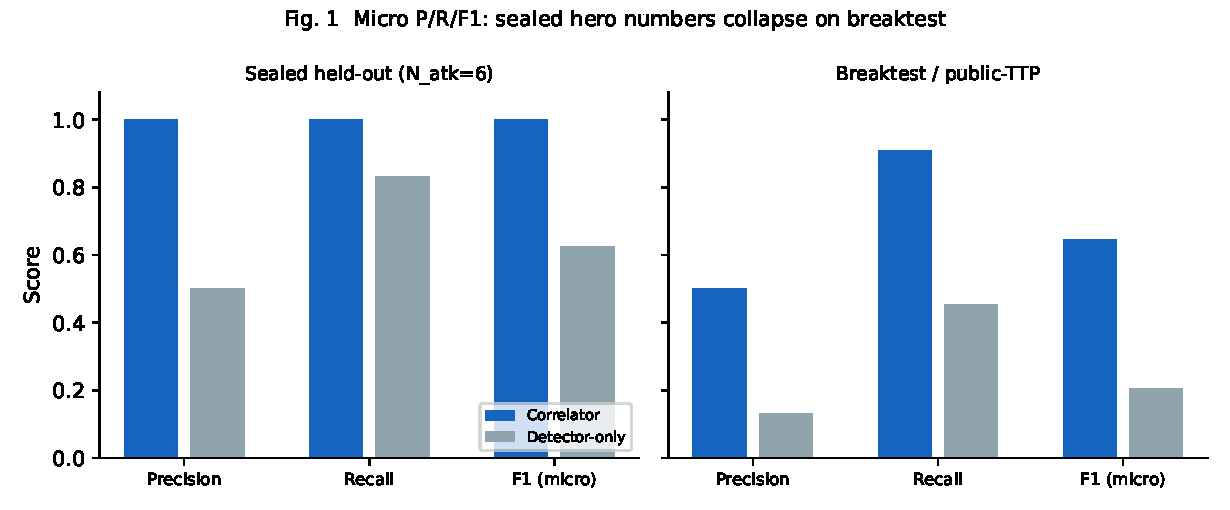
\includegraphics[width=\columnwidth]{figures/fig1_sealed_vs_breaktest.pdf}
\caption{Locked micro P/R/F1. Left: sealed held-out (author GT). Right:
breaktest. Correlator vs detector-only. Sealed hero F1 does not survive B.}
\label{fig:sealed}
\end{figure}

\begin{figure}[!t]
\centering
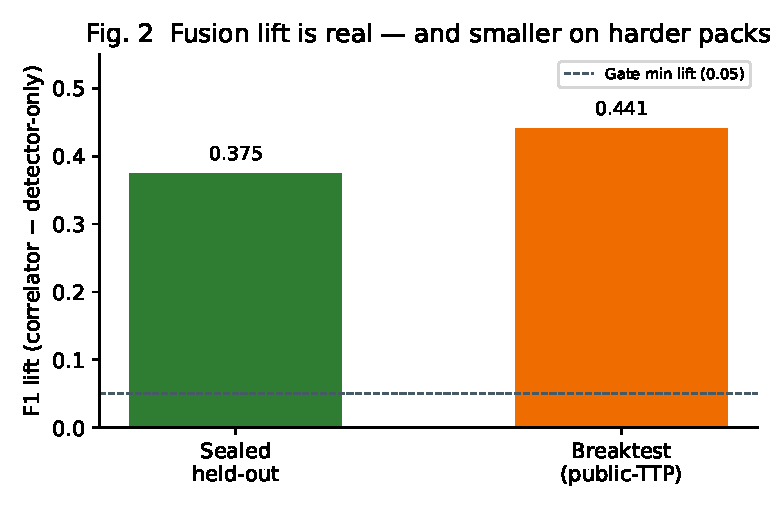
\includegraphics[width=0.92\columnwidth]{figures/fig2_fusion_lift.pdf}
\caption{Fusion lift: sealed $+0.375$; breaktest $+0.441$ (dashed line:
minimum lift $0.05$ used in the non-author check). Lift can grow while
absolute F1 falls.}
\label{fig:lift}
\end{figure}

\begin{table}[!t]
\caption{Protocol~S locked counts (author-generated, sealed).}
\label{tab:sealed}
\centering
\scriptsize
\begin{tabular}{@{}lcccc@{}}
\toprule
Arm & $P$ & $R$ & $F1$ & TP/FP/FN \\
\midrule
Correlator & $1.00$ & $1.00$ & $\mathbf{1.00}$ & $6/0/0$ \\
Detector-only & $0.50$ & $0.833$ & $0.625$ & $5/5/1$ \\
B1 single-host & $0.00$ & $0.00$ & $0.00$ & $0/1/6$ \\
\bottomrule
\end{tabular}
\end{table}

Benign FCR~$=0.00$ at $N_{\mathrm{ben}}{=}6$.
Perfect correlator F1 is \emph{necessary but not sufficient}.
Detector-only $0.625$ shows fusion still matters on this set; B1 shows that
naive single-host aggregation recovers nothing.
Fig.~\ref{fig:fam} shows per-family sealed correlator F1---still synthetic
authorship.

\begin{figure}[!t]
\centering
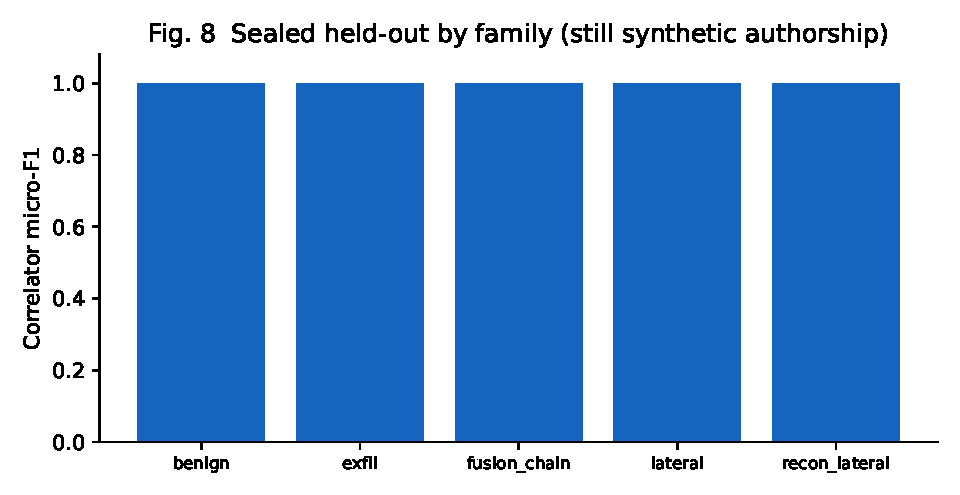
\includegraphics[width=\columnwidth]{figures/fig8_sealed_families.pdf}
\caption{Sealed correlator F1 by family. Still synthetic authorship---do not
read as OTRF independence.}
\label{fig:fam}
\end{figure}

\paragraph{Interpretation.}
Protocol~S answers ``does the pipeline work under its own sealed packs?''
It does not answer ``is field-scope prose warranted?''

\subsection{Protocol B --- breaktest / public-TTP}
\label{sec:breaktest}

\begin{table}[!t]
\caption{Protocol~B locked counts (author-assembled manifests; public TTP IDs).}
\label{tab:break}
\centering
\scriptsize
\begin{tabular}{@{}lcccc@{}}
\toprule
Arm & $P$ & $R$ & $F1$ & TP/FP/FN \\
\midrule
Correlator & $0.500$ & $0.909$ & $\mathbf{0.645}$ & $10/10/1$ \\
Detector-only & $0.132$ & $0.455$ & $0.204$ & $5/33/6$ \\
Lift & \multicolumn{4}{c}{$+0.441$} \\
\bottomrule
\end{tabular}
\end{table}

Absolute F1 drops $1.00\rightarrow 0.645$.
Precision halves ($1.00\rightarrow 0.50$).
False positives rise from $0$ to $10$ on the correlator arm; detector-only
false positives explode to $33$.
This is the first honest hardness signal: fusion lift remains large
($+0.441$), but absolute quality is no longer a hero number.

\paragraph{Do not confuse lift with readiness.}
Fig.~\ref{fig:lift} shows breaktest lift can \emph{exceed} sealed lift while
absolute F1 falls.
A reader who quotes only lift can still overclaim.

\subsection{Protocol O --- broad OTRF (external)}
\label{sec:otrf}

\begin{figure}[!t]
\centering
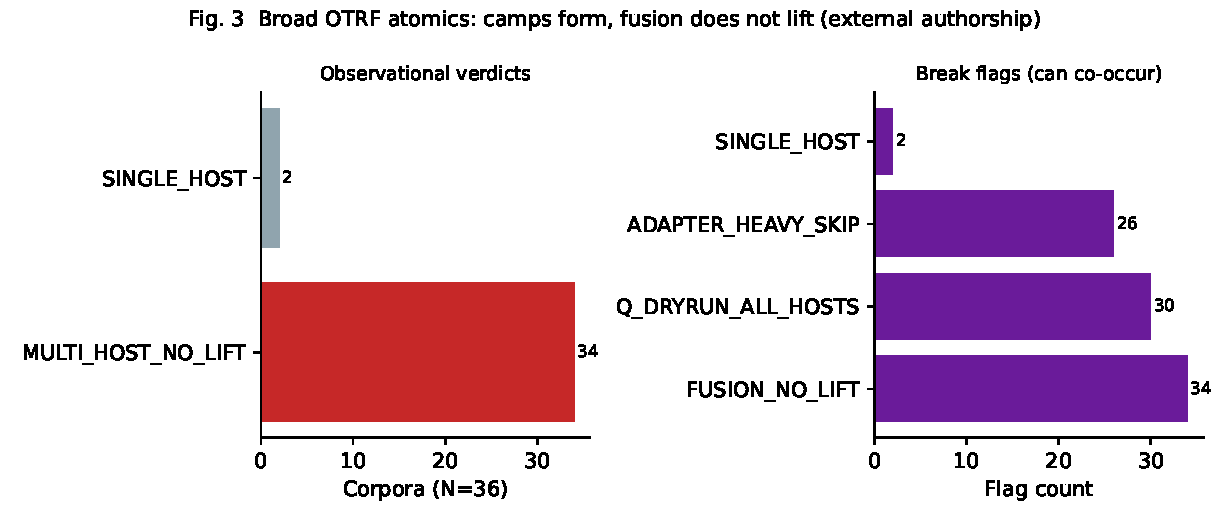
\includegraphics[width=\columnwidth]{figures/fig3_otrf_broad.pdf}
\caption{Protocol~O ($N{=}36$ external). Left: observational verdicts
($34$ no-lift). Right: co-occurring break flags including $30\times$
fleet-wide quarantine dry-run.}
\label{fig:otrf}
\end{figure}

Honest reading: multi-host campaigns \emph{form} on public captures; fusion
does \emph{not} beat detector-only host coverage on this atomic set
($34/36$ \textsc{MultiHostNoLift}; $2$ \textsc{SingleHost}).
Break flags co-occur: $34\times$ fusion-no-lift, $30\times$ quarantine dry-run
proposing essentially all hosts, $26\times$ heavy adapter skip.
Those failures drove the correlator and quarantine fixes measured in
Protocol~A---not a retroactive rewrite of Fig.~\ref{fig:otrf}.

\paragraph{Why this is the independence headline.}
Protocol~O packs are externally authored.
They are still lab purple-team captures, not enterprise estates---but they are
not Corvex-written fleet manifests.
Leading with Fleet20 would reverse the authorship hierarchy
(Section~\ref{sec:secondary}).

\subsection{Protocol A --- aggressive compounds}
\label{sec:aggressive}

\begin{figure}[!t]
\centering
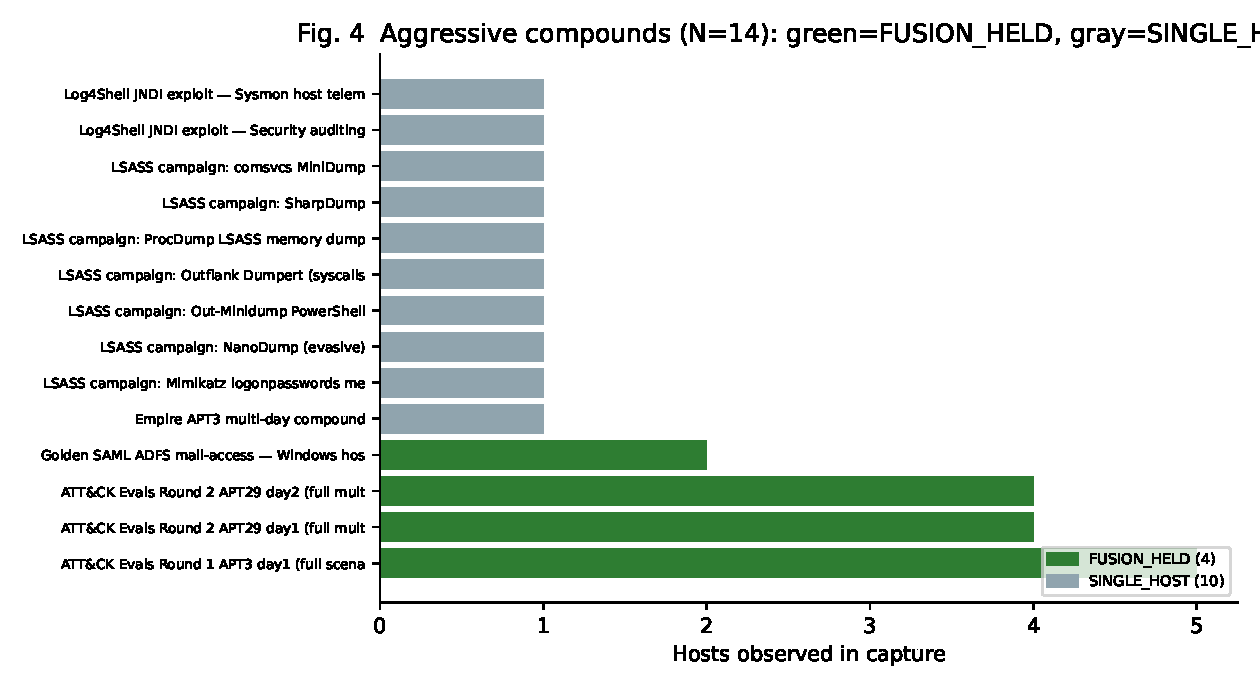
\includegraphics[width=\columnwidth]{figures/fig4_aggressive.pdf}
\caption{Protocol~A ($N{=}14$). Green bars: \textsc{FusionHeld} (4). Gray:
\textsc{SingleHost} (10). $x$-axis: hosts observed in capture.}
\label{fig:agg}
\end{figure}

\begin{figure}[!t]
\centering
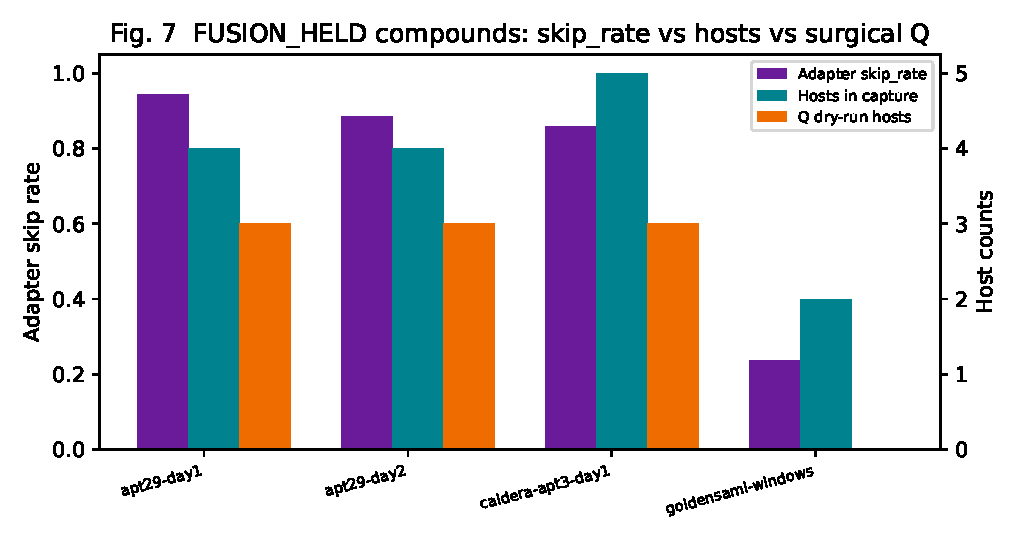
\includegraphics[width=\columnwidth]{figures/fig7_adapter_skip.pdf}
\caption{Even held compounds: adapter \texttt{skip\_rate} (purple) vs hosts
(teal) vs surgical Q dry-run host count (orange). APT29 remains
allowlist-blind on most raw events.}
\label{fig:skip}
\end{figure}

\begin{table}[!t]
\caption{Protocol~A held compounds (locked). Skip rates from adapter logs.}
\label{tab:held}
\centering
\scriptsize
\begin{tabular}{@{}lrrrr@{}}
\toprule
Corpus & Hosts & Events & Skip rate & Q hosts \\
\midrule
APT29 day1 & 4 & 10\,980 & 0.944 & 3 \\
APT29 day2 & 4 & 67\,693 & 0.885 & 3 \\
Caldera APT3 day1 & 5 & 14\,423 & 0.859 & 3 \\
Golden SAML & 2 & 29 & 0.237 & 0 \\
\bottomrule
\end{tabular}
\end{table}

Held set: APT29 day1, APT29 day2, Caldera APT3 day1, Golden SAML
(Table~\ref{tab:held}).
The remaining 10 corpora are \textsc{SingleHost} (Empire APT3 compound,
LSASS$\times$7, Log4Shell$\times$2)---fusion not testable.
After ambient micro-exfil poison, hop peers via WorkstationName, no recon
host-union, and surgical cut-point quarantine, fleet-wide Q dry-run and
\textsc{MultiHostNoLift} counts on this aggressive set are zero in the locked
rollup---but adapter skip rates on APT29 remain $0.86$--$0.94$.

\paragraph{Saturated-lab honesty.}
On saturated 4--5 host labs, host-coverage lift can be definitionally zero when
both arms already cover all hosts.
\textsc{FusionHeld} here means consolidation + surgical Q (not fleet-wide
spray), not ``more hosts than detector on every atomic.''

\subsection{Protocol L --- live laptop replay}
\label{sec:live}

\begin{figure}[!t]
\centering
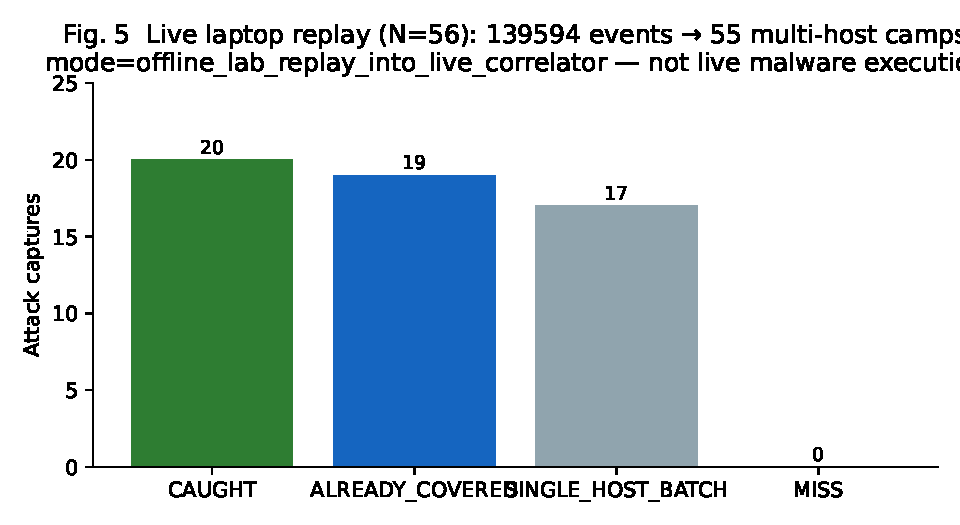
\includegraphics[width=\columnwidth]{figures/fig5_live_catch.pdf}
\caption{Protocol~L catch labels from locked live stress JSON.
Mode=\texttt{offline\_lab\_replay\_into\_live\_correlator}.
$139{,}594$ events $\rightarrow$ $55$ multi-host camps. Not live malware.}
\label{fig:live}
\end{figure}

\begin{table}[!t]
\caption{Protocol~L catch rollup ($N{=}56$).}
\label{tab:live}
\centering
\scriptsize
\begin{tabular}{@{}lrl@{}}
\toprule
Label & $N$ & Meaning \\
\midrule
\textsc{Caught} & $20$ & New multi-host bridge / camp growth \\
\textsc{AlreadyCovered} & $19$ & Hosts already in multi-host camps \\
\textsc{SingleHostBatch} & $17$ & Capture has $<2$ hosts \\
\textsc{Miss} & $\mathbf{0}$ & Multi-host capture failed to register \\
\bottomrule
\end{tabular}
\end{table}

Wall time for the locked run is $675$\,s.
Final snapshot: $139{,}594$ events; $55$ multi-host campaigns spanning APT29,
Caldera, Mordor workstation, and Golden SAML hostnames.
\textsc{AlreadyCovered} is not failure: later captures land inside camps grown
by earlier ones.
\textsc{Miss}${}=0$ must not be read as ``caught live malware on the laptop.''

\begin{figure}[!t]
\centering
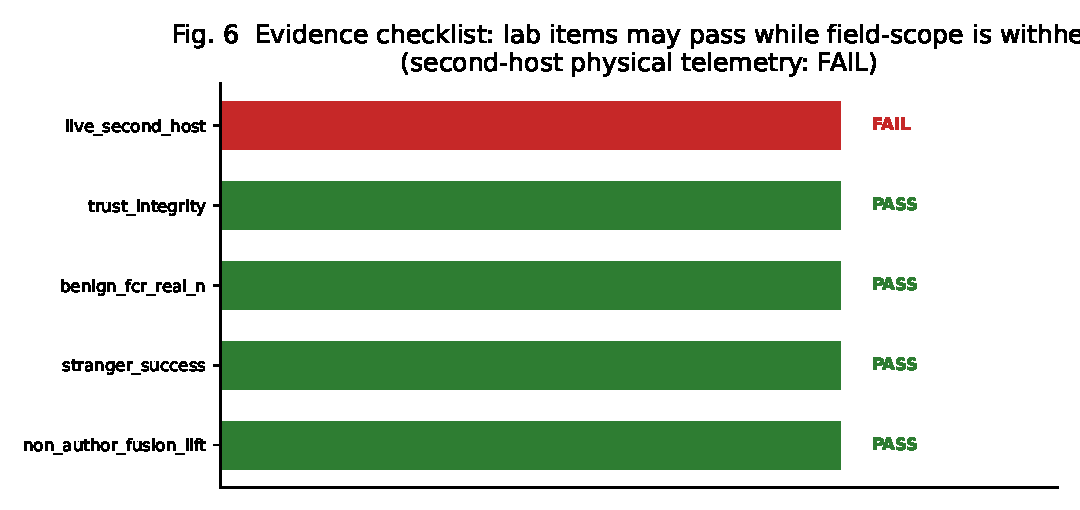
\includegraphics[width=\columnwidth]{figures/fig6_claim_gates.pdf}
\caption{Evidence checklist (locked reports). Four items pass; second-host
physical telemetry fails. Lab scores may be green while field-scope prose
remains unwarranted.}
\label{fig:gates}
\end{figure}

\subsection{Named failure mechanisms}
\label{sec:failures}

\begin{table}[!t]
\caption{Mechanism table (synthetic unless noted). Status as of locked reports.}
\label{tab:fail}
\centering
\scriptsize
\begin{tabular}{@{}p{0.95in}p{1.55in}p{0.7in}@{}}
\toprule
Mode & Mechanism & Status \\
\midrule
DHCP split-brain & Distinct \texttt{host\_id} strings & Held \\
Day-scale sleeper & 1\,h resume fragmented chains & Held \\
Shared svc glue & Time window glued hop islands & Unit held \\
Egress bury & CDN-like dst fanout & Mixed / Broke cells \\
DNS-only C2 & No Sysmon EID~22 & Honest gap \\
Fleet-wide Q & Recon union + all-host spray & Fixed \\
Ambient metadata & \texttt{169.254.169.254}/Azure wire & Fixed \\
APT29 skip & Channel allowlist & Remaining \\
\bottomrule
\end{tabular}
\end{table}

Earlier packaging named breaks without mechanisms.
Table~\ref{tab:fail} is the condensed WHY list.
Egress bury remains a live edge on some intensive author cells even after unit
poison tests pass---another reason not to lead with author-fleet headlines.

% =====================================================================
\section{Secondary Author Fleets (Not Independence)}
\label{sec:secondary}
% =====================================================================

Author-written fleets are useful for mechanism debugging.
They are the wrong headline for independence.

\paragraph{Fleet20.}
Locked rollup: $20/20$ \textsc{Held}, fragile rate $0.05$ among held cells.
Never report bare $20/20$ without the fragile rate.

\paragraph{Intensive multifactor.}
Locked rollup: \textsc{Held}~$23$ (fragile~$5$), \textsc{Partial}~$2$,
\textsc{Broke}~$3$ (all \texttt{exfil\_bury} cells), errors~$0$.
These packs are in-repo purple-team sketches under
\texttt{labs/breaktest/manifests/fleet-intensive}.

\paragraph{Placement rule.}
If an abstract mentions Fleet20 before OTRF, authorship hierarchy is inverted.
This paper places $F_{\mathrm{sec}}$ after Protocols O/A/L by design.

% =====================================================================
\section{Discussion: Withheld Field-Scope Sentence}
\label{sec:vignette}
% =====================================================================

\paragraph{Example of an unwarranted upgrade.}
``Corvex works on real multi-host attacks in enterprise networks and is ready
for production SOC use.''
Under the locked evidence checklist, second-host physical telemetry is missing,
so that sentence is out of scope for this manuscript.
The standing scope remains synthetic ATT\&CK-shaped fleets and externally
authored lab purple-team captures.

\paragraph{What lab-coherence buys.}
Sealed F1~$1.00$, breaktest lift $+0.441$, stranger dry-run attestation, and
integrity probes support statements of the form: \emph{under these protocols,
fusion beats detector-only and ingest rejects bad HMAC}.
They do not buy enterprise readiness.

\paragraph{Reusable checklist (for other detectors).}
\begin{enumerate}
\item Authorship column on every scoreboard.
\item Micro-F1 only for headlines ($2PR/(P{+}R)$ from pooled counts).
\item Always ablate fusion (or the analogous upgrade).
\item External corpora before self-fleets.
\item Name failure mechanisms---never status labels alone.
\item Separate lab-coherent scores from field-scope warrant.
\item Quarantine cut-points (fleet-wide dry-run is not ready).
\item Replay honesty (replay $\neq$ live implant catch).
\end{enumerate}

\paragraph{Implications for detection papers.}
Negative or partial results on external corpora are not defects to bury under
sealed F1.
They are the content that makes the sealed number interpretable.

% =====================================================================
\section{Related Work}
\label{sec:related}
% =====================================================================

\subsection{Closed-world evaluation}
Sommer and Paxson warn that closed-world intrusion evaluations overstate
detector quality~\cite{sommer_paxson_2010}.
The analogy here is \emph{sealed-pack optimism}: a separable held-out pack
proves wiring and is then screenshotted as field evidence.

\subsection{Datasets and purple-team corpora}
Surveys of network intrusion datasets emphasize authorship, labeling, and
leakage risks~\cite{ring_2019_survey}.
OTRF/Security-Datasets and ATT\&CK Evaluations provide external purple-team
captures used here as independence stress~\cite{otrf_mordor,attack_evals,caldera}.
Atomic Red Team supplies public TTP IDs referenced by breaktest
manifests~\cite{atomic_red_team}.

\subsection{Reporting discipline}
Model cards and explicit release criteria motivate separating score tables from
field-scope prose~\cite{van_leeuwen_model_cards}.
CSET-style venues solicit metrics, datasets, and experimental
discipline~\cite{cset_charter}.
We package these practices into one open correlator evaluation with locked
figures---not a novel learning algorithm.

\subsection{Negative results}
Reliability and security tooling have structural incentives to publish hero
lab scores and soft-pedal external drops.
We write against that incentive by leading with Protocol~O/A and by withholding
field-scope sentences when second-host evidence is absent.

% =====================================================================
\section{Threats to Validity}
\label{sec:threats}
% =====================================================================

\paragraph{Internal.}
Sealed and breaktest ground truth are author-defined; micro-F1 inherits those
labels.
Observational OTRF verdicts avoid inventing GT F1 but depend on adapter
allowlists and host-coverage definitions.

\paragraph{External.}
OTRF and ATT\&CK Evals captures are lab purple-team, not enterprise estates.
Live replay is not live malware execution.
Second-host physical telemetry is missing.

\paragraph{Construct.}
\textsc{FusionHeld} on saturated fleets is not identical to positive
host-coverage lift.
Catch labels on Protocol~L mix growth and already-covered states; both are
reported.

\paragraph{Conclusion.}
The paper's primary claim is about evaluation hygiene and scope boundaries,
which is less sensitive to enterprise transfer than a ``beats commercial EDR''
claim would be---a claim we do not make.

% =====================================================================
\section{Limitations}
\label{sec:limits}
% =====================================================================

Sealed $N_{\mathrm{atk}}{=}6$ is modest; larger $N$ reduces variance but does
not create field validity.
Breaktest remains author-assembled.
OTRF is external but still lab purple-team.
\textsc{FusionHeld} $\neq$ host-coverage lift on every atomic.
Adapter skip rates on APT29 remain high.
No second physical Windows host yet---field-scope sentences withheld.
Home-lab benign PASS/FAIL against pre-committed bars deferred.
Live stress is replay.
Author fleets remain secondary.

% =====================================================================
\section{Conclusion}
\label{sec:conclusion}
% =====================================================================

Sealed F1~$1.00$ is not a field claim.
Under locked protocols, Corvex shows a measurable drop on breaktest, honest
no-lift on broad OTRF, partial holds on hardest compounds with residual adapter
blindness, and zero-miss live \emph{replay}, while second-host evidence remains
absent.
The portable lesson is the protocol ladder and authorship hierarchy: seal,
ablate, prefer external corpora, name mechanisms, and withhold field-scope
prose until the stated evidence exists.
Future work: second-host attestation and benign baseline PASS/FAIL---without
softening scope ahead of evidence.

\section*{Artifact Availability}
\url{https://github.com/Siddarthb07/corvex}; figures:
\texttt{docs/paper/figures/}; lockfile:
\texttt{docs/paper/NUMBERS\_LOCKED.json}; rebuild figures:
\texttt{python scripts/render\_paper\_figures.py}; rebuild PDF:
\texttt{python scripts/build\_journal\_paper\_pdf.py}.

\section*{Ethics}
No live malware execution; OTRF sanitized before local storage; quarantine
dry-run by default; TLP:CLEAR public purple-team data~\cite{first_tlp}.

\bibliographystyle{IEEEtran}
\bibliography{refs}

\appendix[Reproduce]
\label{app:repro}
\begin{footnotesize}
\begin{verbatim}
pip install -e ".[dev]"
corvex seal-day0 --force && corvex eval --split heldout
corvex score-non-author
python scripts/fetch_opensource_corpora.py --full
python scripts/run_opensource_attack_eval.py
python scripts/fetch_opensource_corpora.py --aggressive
python scripts/run_opensource_attack_eval.py --aggressive
python scripts/run_live_opensource_stress.py --dash
python scripts/render_paper_figures.py
\end{verbatim}
\end{footnotesize}

\appendix[Authorship Tiers]
\label{app:tiers}
\begin{table}[!h]
\caption{Authorship tiers used throughout.}
\label{tab:tiers}
\centering
\scriptsize
\begin{tabular}{@{}lp{2.2in}@{}}
\toprule
Tier & Meaning \\
\midrule
Author-synthetic & Sealed generators; Corvex GT \\
Author-breaktest & In-repo manifests; public TTP IDs \\
External-lab & OTRF / ATT\&CK Evals purple-team \\
Stranger-enterprise & Not claimed in this manuscript \\
\bottomrule
\end{tabular}
\end{table}

\balance
\end{document}
